\documentclass[12pt]{article}
\usepackage[utf8]{inputenc}
\usepackage[T1]{fontenc}
\usepackage[a4paper, total={6in, 9in}]{geometry}
\usepackage{graphicx}
\graphicspath{ {./images/output/} }
\usepackage{caption}
\usepackage[english]{babel}
\usepackage{titling}
\usepackage{float}
\usepackage{amsmath}
\usepackage{minted}
\usepackage{multicol}
% \usepackage{array}
% \usepackage{setspace}
% \usepackage{placeins}
\usepackage{parskip}

% \usepackage{lipsum}

\title{Implementation of Half Adder Circuit Using CMOS in Microwind}
\author{}
\date{}

\pagenumbering{gobble}
\begin{document}
\vspace*{\fill}
\begin{center}

    \emph{Heaven's Light is Our Guide} \\
    \textbf{Rajshahi University of Engineering and Technology} \\

    \begin{figure}[H]
        \centering
        
\includegraphics[scale=.34]{images/RUET_logo.png}
        \label{fig:ruet_logo}
    \end{figure}
    \vspace{5mm}

    \textbf{Course Code}\\
    ECE 4128\\
    \vspace{3mm}
    \textbf{Course Title}\\
    VLSI Design

    \vspace{5mm}
    \textbf{Experiment Date:} {July 4, 2025},\\
    \textbf{Submission Date:} {August 11, 2025}\\

    \vspace{5mm}
    \textbf{Lab Report 2: \\
        Implementation of NMOS Ratio-less Inverter.}

    \vspace{15mm}

    \begin{tabular}{c|c}
        \textbf{Submitted to} & \textbf{Submitted by} \\
        Moloy Kumar Ghosh     &                       \\
        Lecturer              &                       \\
        Dept of ECE, RUET     & Md. Tajim An Noor     \\
        \&                    & Roll: 2010025         \\
        Md. Faysal Ahamed     &                       \\
        Lecturer              &                       \\
        Dept of ECE, RUET     &                       \\
    \end{tabular}

\end{center}
\vspace*{\fill}


\pagebreak

\tableofcontents

\pagebreak
\pagenumbering{arabic}
\maketitle

\section*{Theory}
\addcontentsline{toc}{section}{Theory}
A half adder is a combinational logic circuit that adds two single‑bit binary numbers A and B and produces two outputs: Sum (S) and Carry (C). It performs the least‑significant‑bit addition without an incoming carry. The signals have the following meanings:
\begin{itemize}
  \item A, B: single‑bit binary inputs to be added.
  \item Sum (S): the least‑significant bit of the addition result.
  \item Carry (C): the carry‑out bit (1 if the sum exceeds 1 and must be carried to the next higher bit).
\end{itemize}

The half‑adder logic and practical CMOS realizations are discussed in standard texts on digital and VLSI design\cite{weste2011cmos,rabaey2003digital,sedra2015microelectronic}.

Boolean expressions
\[
  S = A \oplus B = A\overline{B} + \overline{A}B
\]
\[
  C = A \cdot B
\]
These expressions and their transistor‑level mappings (XOR implemented via complementary networks or transmission gates, AND via NAND+inverter or static AND) are treated in detail in the cited books\cite{rabaey2003digital,weste2011cmos}.

\begin{table}[H]
  \centering
  \begin{tabular}{|c c |c |c|}
    \hline
    A & B & Sum (S) & Carry (C) \\
    \hline
    0 & 0 & 0       & 0         \\
    0 & 1 & 1       & 0         \\
    1 & 0 & 1       & 0         \\
    1 & 1 & 0       & 1         \\
    \hline
  \end{tabular}
  \caption*{Truth table of Half Adder (definition after \cite{sedra2015microelectronic})}
\end{table}

Logic (gate‑level) circuit:
\begin{itemize}
  \item Sum: XOR gate taking inputs A and B.
  \item Carry: AND gate taking inputs A and B.
\end{itemize}
Both inputs A and B feed the XOR (for S) and the AND (for C) so the block diagram is the two inputs branching to these two gates.

\begin{figure}[H]
  \centering
  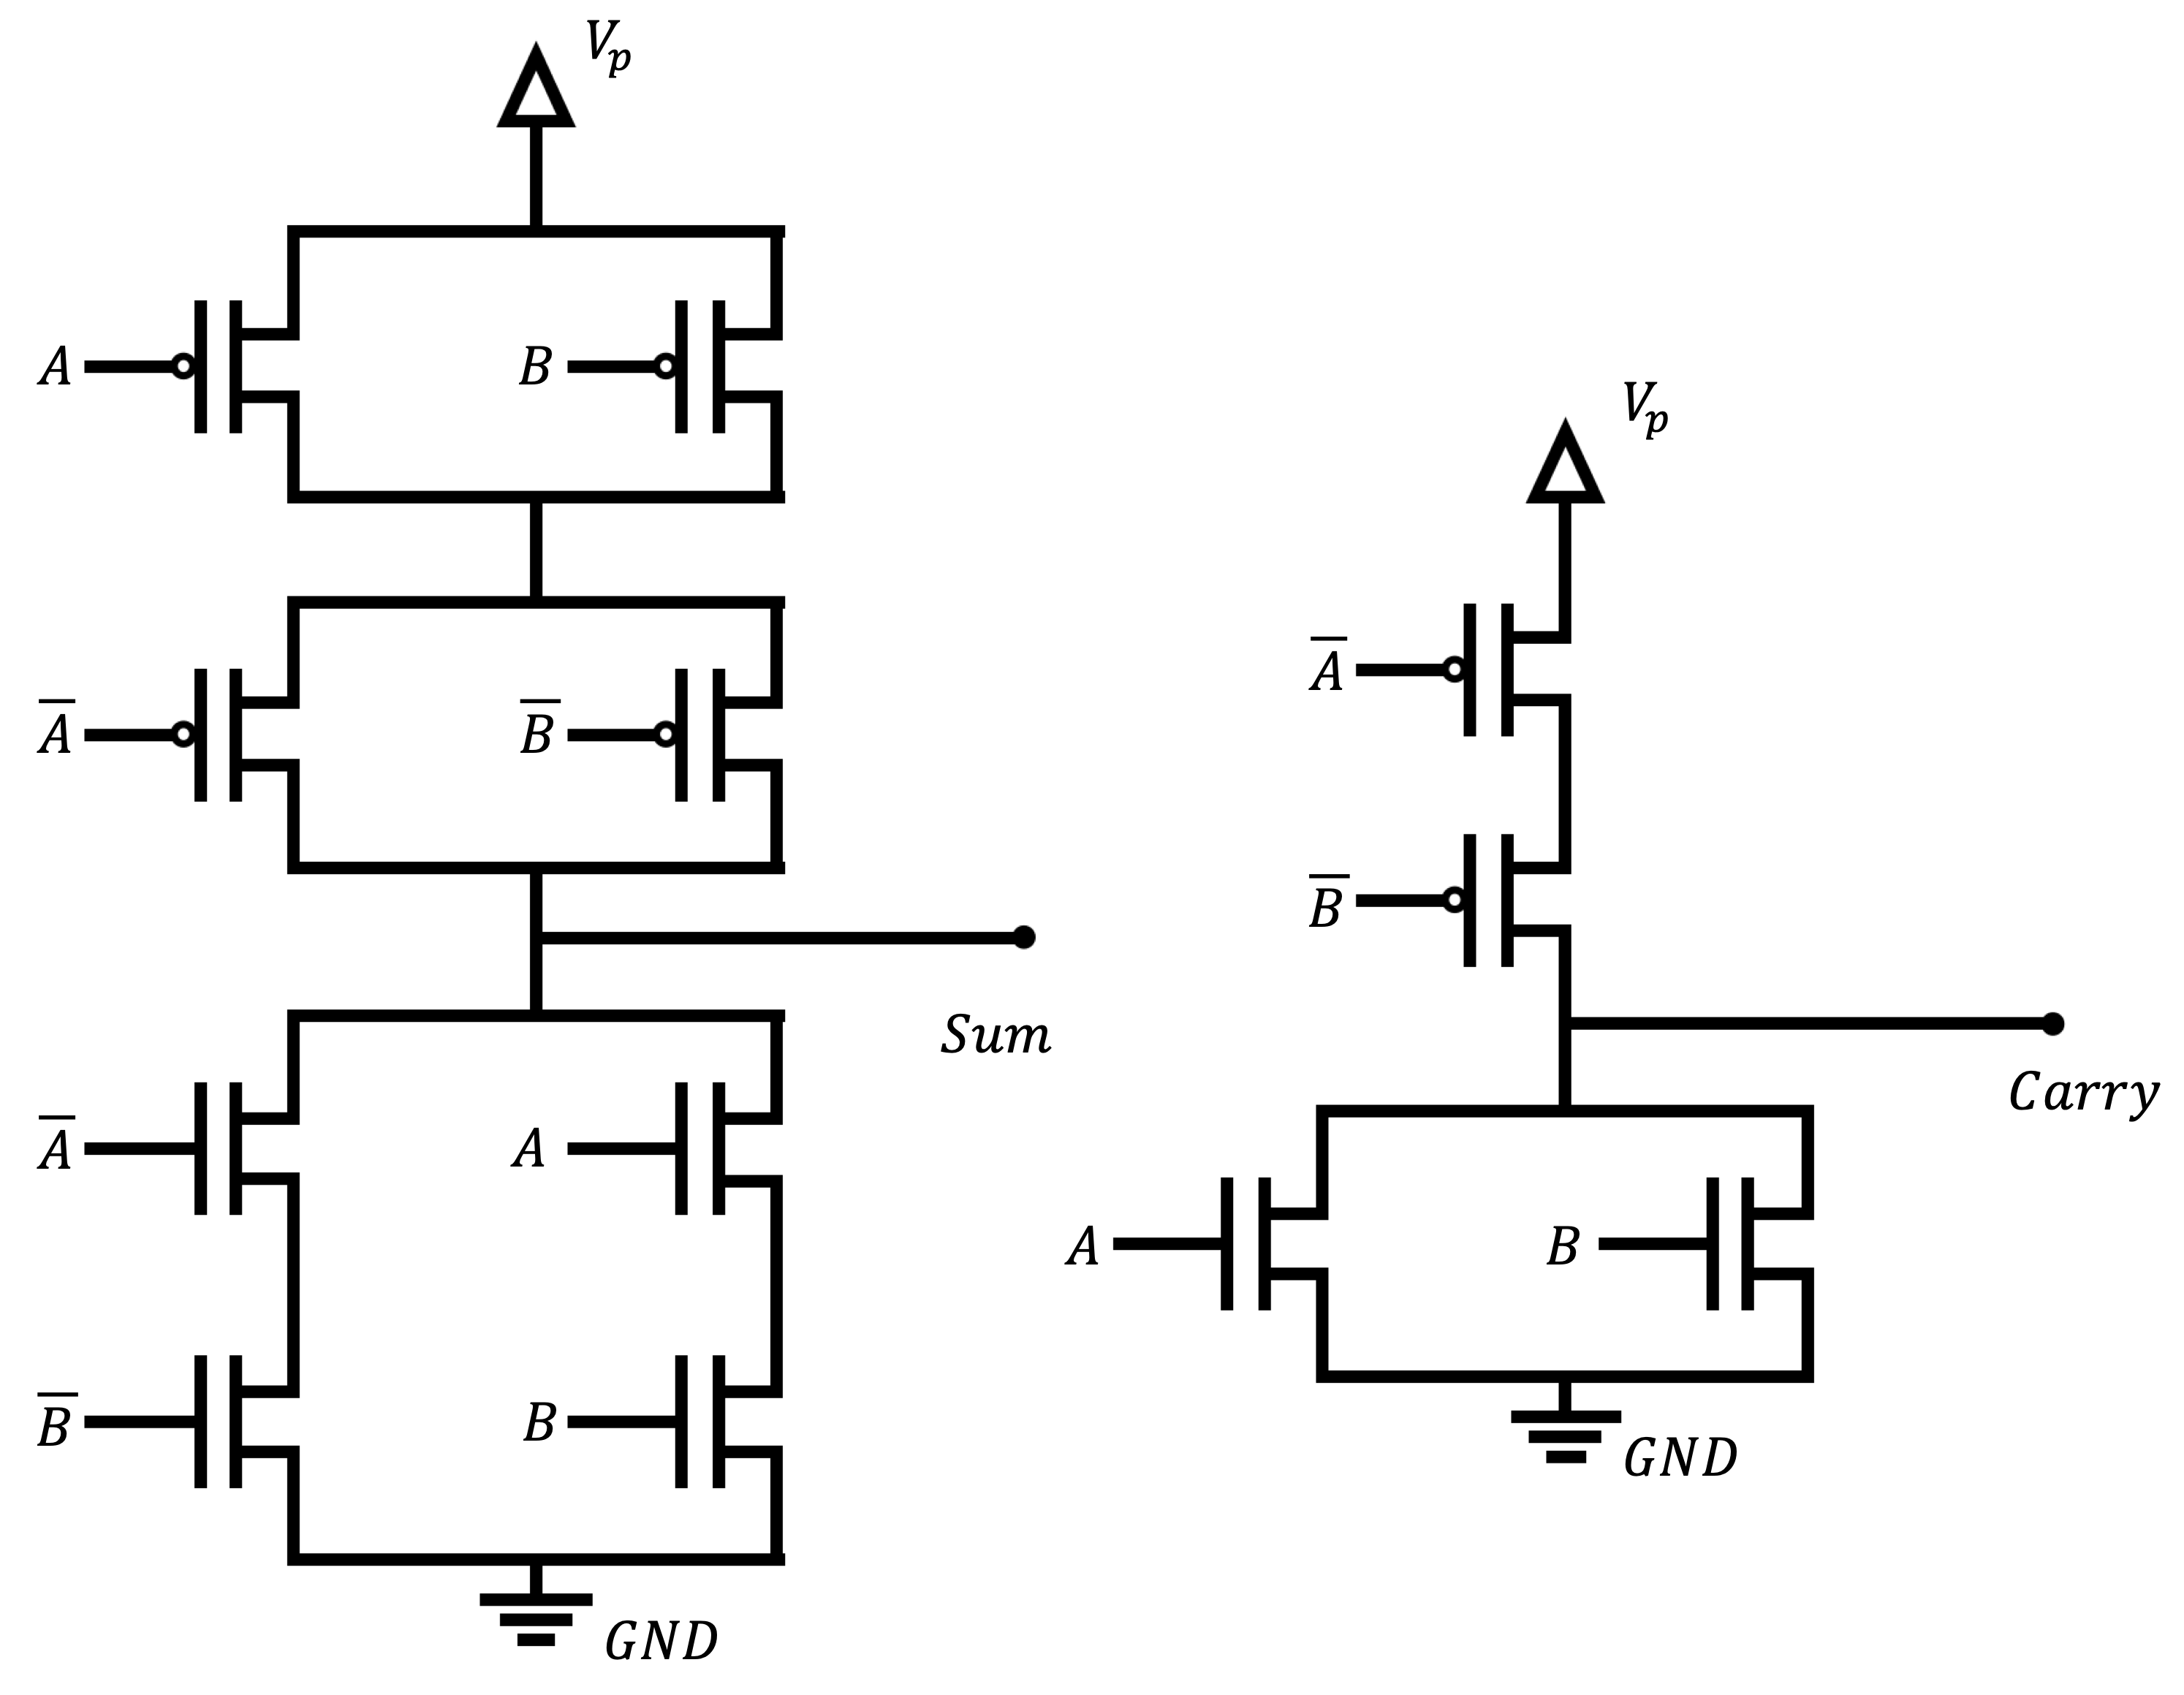
\includegraphics[width=.7\textwidth]{ckt.png}
  \caption{CMOS Circuit Diagram of Half Adder}
\end{figure}

CMOS implementation\cite{BibEntry2025Oct}:
\subsection*{CMOS implementation}
\addcontentsline{toc}{subsection}{CMOS implementation}

Sum (XOR)
\[
  S = A \oplus B = \overline{A}B + A\overline{B}
\]
Complement (output low condition), obtained by De Morgan:
\[
  \overline{S} = \overline{\overline{A}B + A\overline{B}}
  = (A + \overline{B})(\overline{A} + B)
  = AB + \overline{A}\,\overline{B}\quad\text{(XNOR)}
\]
Implementation mapping:
\begin{itemize}
  \item nMOS pull-down network (implements $\overline{S}$): two parallel branches --- one branch is nMOS($A$) in series with nMOS($B$); the other branch is nMOS($\overline{A}$) in series with nMOS($\overline{B}$). (If complementary signals $\overline{A}$, $\overline{B}$ are not available, provide inverters or realize XOR with transmission gates.)
  \item pMOS pull-up network (dual of $\overline{S}$): series combination of two parallel pairs, i.e. (pA $\parallel$ p$\overline{B}$) in series with (p$\overline{A}$ $\parallel$ pB). This network pulls the output high when $\overline{S}=0$.
\end{itemize}

Carry (AND)\\
Equation for Carry (Pull-up network):
\[
  C = A\cdot B
\]
Complement (for the nMOS pull‑down network), by De Morgan:
\[
  \overline{C} = \overline{A\cdot B} = \overline{A} + \overline{B}
\]



\section*{Used Tools}
\addcontentsline{toc}{section}{Used Tools}
\begin{itemize}
  \item Microwind
  \item MS Word
  \item MS PowerPoint
  \item \LaTeX
\end{itemize}

\section*{Circuit Schematic in Microwind}
\addcontentsline{toc}{section}{Circuit Schematic in Microwind}

\begin{figure}[H]
  \centering
  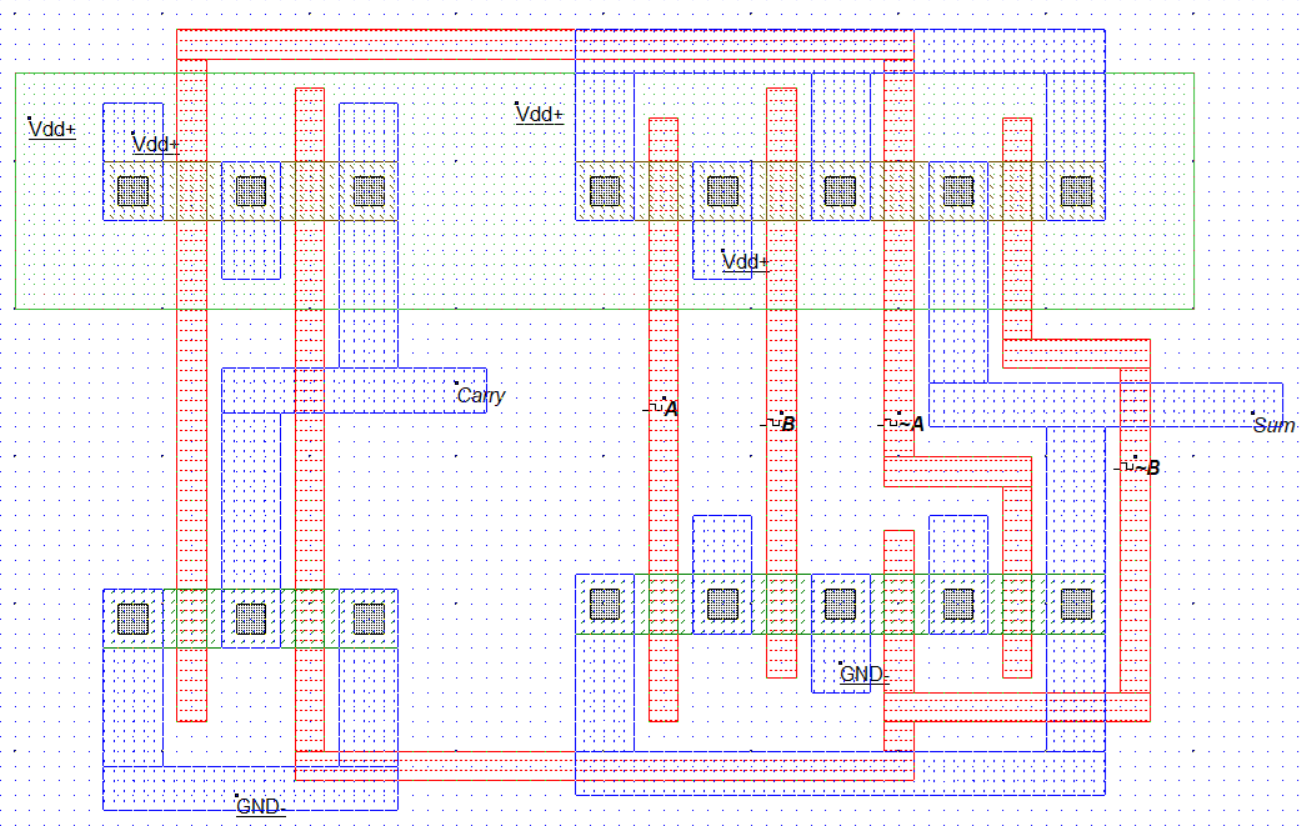
\includegraphics[width=\textwidth]{mCkt.png}
  \caption{Half Adder Circuit Schematic in Microwind}
\end{figure}

\section*{Output}
\addcontentsline{toc}{section}{Output}

\begin{figure}[H]
  \centering
  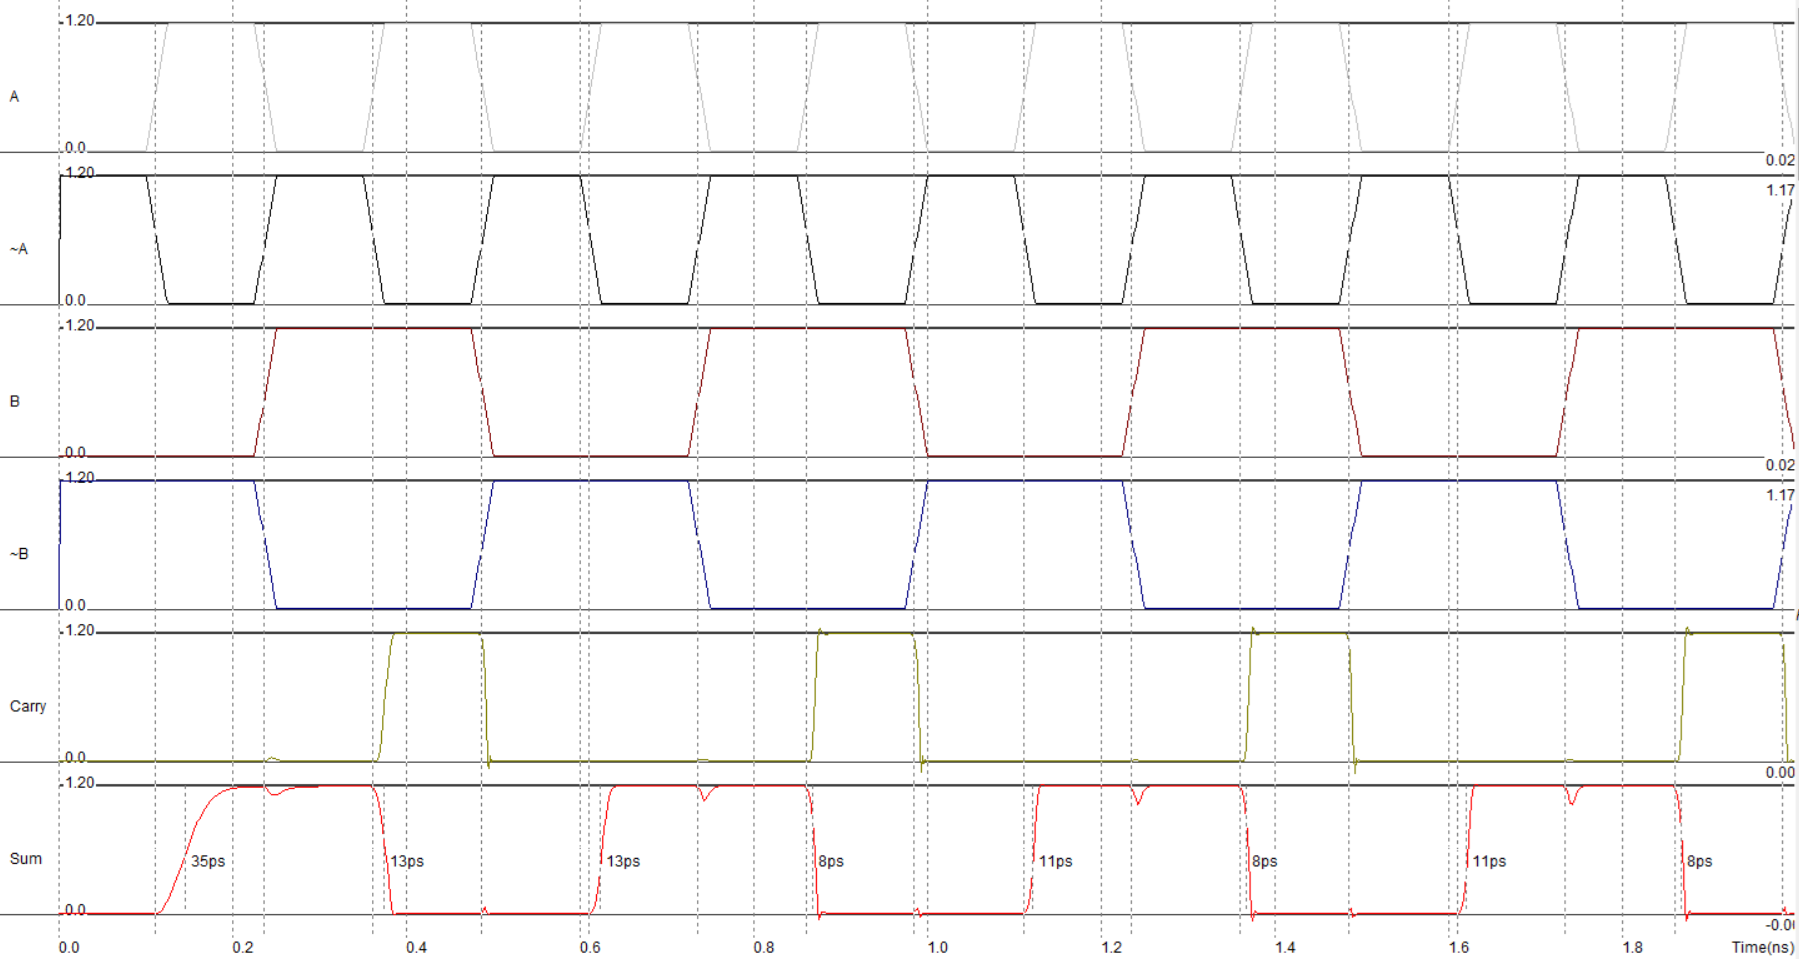
\includegraphics[width=\textwidth]{output.png}
  \caption{Sum \& Carry Output Waveform of Half Adder Circuit}
\end{figure}

\subsection*{Output Analysis}
\addcontentsline{toc}{subsection}{Output Analysis}
\begin{enumerate}
  \item Testbench and signal summary
        \begin{itemize}
          \item Supply: VDD \(\approx\) 1.20\,V (top trace marker).
          \item Inputs: A and B driven with periodic pulses (top traces).
          \item Outputs: Carry (green) and Sum (red). Time base in the plot is nanoseconds; zoomed markers show pulses spaced ~0–2\,ns.
        \end{itemize}

  \item Logic-level correctness
        \begin{itemize}
          \item Carry (\(C=A\cdot B\)): goes high (~1.20\,V) only when both A and B are high; remains near 0\,V otherwise. Example: cycle near 0.3–0.45\,ns both inputs high and Carry rises to VDD.
          \item Sum (\(S=A\oplus B\)): high when exactly one input is high, low when inputs are equal (both 0 or both 1). Sum falls to 0 when both inputs are high while Carry goes high, matching expected half‑adder outputs.
        \end{itemize}
\end{enumerate}

\section*{Discussion}
\addcontentsline{toc}{section}{Discussion}
The implemented half adder ($S=A\oplus B$, $C=A\cdot B$) was simulated in Microwind and matches the truth table: Carry rises only when A and B are high and Sum follows XOR behavior. Waveforms show finite propagation delays and non‑ideal rise/fall times — the XOR (Sum) path is slower due to a larger transistor network, and PMOS devices were widened to better balance rise/fall. Dynamic switching dominates power; buffering the outputs with inverters and using a carefully sized static complementary or transmission‑gate XOR reduces delay and voltage degradation.

Overall the simulation confirms a correct CMOS half adder implementation while highlighting the usual tradeoffs between speed, area (transistor count), and power.

\section*{Conclusion}
\addcontentsline{toc}{section}{Conclusion}
A CMOS half adder was implemented and simulated in Microwind. The circuit produced the expected Sum and Carry waveforms for all input combinations, demonstrating correct logical operation. The exercise illustrates important design considerations for CMOS combinational circuits: choose transistor sizes to balance speed and noise margin, use buffering for improved drive and signal swing, and evaluate power/delay tradeoffs. Future work could measure propagation delay and energy per operation quantitatively, optimize the XOR topology for speed or area, and extend the design to a full adder and multi‑bit adder chains.


\bibliographystyle{IEEEtran}
\renewcommand{\bibname}{References}
\addcontentsline{toc}{section}{References}
\bibliography{ref}

\end{document}
